\section{Các cách biểu diễn mã nguồn}

Có nhiều cách biểu diễn mã nguồn khác nhau đã được phát triển trong lĩnh vực phân tích chương trình và thiết kế trình biên dịch.
Mục đích chung của các cách biểu diễn là giải thích các thuộc tính của chương trình.
Các kiểu biểu diễn chủ yếu ở dưới dạng cấu trúc dữ liệu cây và đồ thị.
Khóa luận này sẽ tập trung vào đồ thị CPG, trong đó đồ thị CPG là dạng đồ thị được hợp thành từ cây AST, đồ thị CFG và đồ thị PDG.

\subsection{Cây cú pháp trừu tượng}

Cây cú pháp trừu tượng (Abstract Syntax Tree) \cite{zhang2019novel} là dạng biểu diễn đầu tiên của mã nguồn, và là cơ sở cho các dạng biểu diễn tiếp theo.
AST không chứa tất cả cú pháp chi tiết nhưng vẫn thể hiện được quan hệ của các biểu thức, mệnh đề trong mã nguồn.
AST giúp trừu tượng hóa các phần chi tiết của mã nguồn và chỉ giữ lại những thông tin cần thiết để trình biên dịch hiểu cấu trúc của chương trình.
AST là một cây cấu trúc phân cấp, nút trong gọi là toán tử bao gồm biểu thức và mệnh đề, các nút lá gọi là toán hạng bao gồm các biến và ký tự.
AST được áp dụng cho phân tích cấu trúc, biến đổi cấu trúc hoặc phát hiện các đoạn mã cấu trúc giống nhau \cite{yamaguchi2012generalized}.
Tuy nhiên nó không sử dụng được cho các phân tích chuyên sâu hơn bởi vì AST không chứa thông tin về luồng điều khiển hoặc phụ thuộc dữ liệu của chương trình.
Hình \ref{img:c2_ast} biểu diễn một cây AST tương ứng với một đoạn mã nguồn trong Rust.

\begin{figure}[H]
  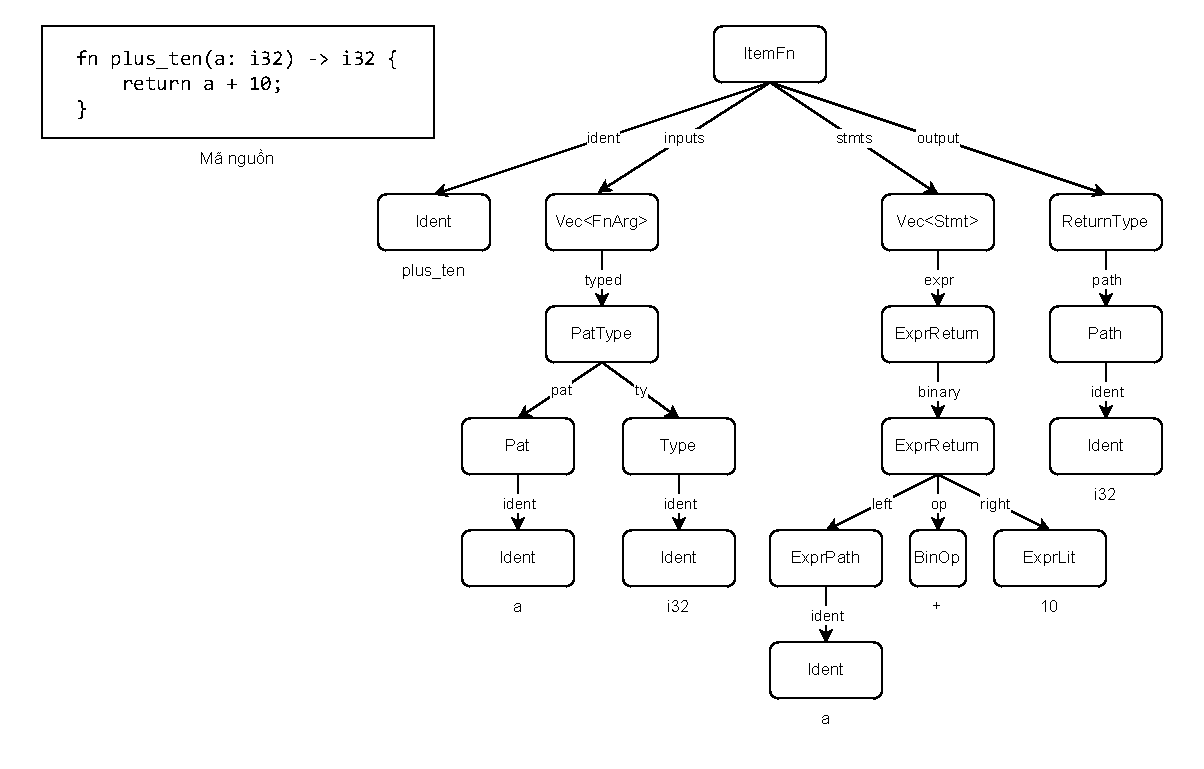
\includegraphics[width=1\columnwidth]{figures/c2/c2_ast.drawio.pdf}
  \centering
  \caption{Ví dụ về cây AST cho mã nguồn Rust.}
  \label{img:c2_ast}
\end{figure}

\subsection{Đồ thị luồng điều khiển}

Đồ thị luồng điều khiển (Control Flow Graph) \cite{yan2019classifying} là đồ thị có hướng, mô tả thứ tự thực thi của các mệnh đề và điều kiện để một mệnh đề được thực thi.
Các nút là các mệnh đề hoặc mệnh đề điều kiện, được nối với nhau bằng các cạnh có hướng, thể hiện thứ tự điều khiển giữa các nút.
Một nút là mệnh đề thì có 1 cạnh ra.
Nếu một nút là mệnh đề điều kiện thì sẽ có 2 cạnh ra, bao gồm một cạnh điều khiển khi điều kiện đúng và một cạnh điều khiển khi điều kiện sai.
CFG được sử dụng cho nhiều ứng dụng phân tích ngữ cảnh, phân tích mã độc hại \cite{gascon2013structural}, định hướng cho công cụ kiểm thử mờ \cite{sparks2007automated}.
Tuy nhiên, CFG không chứa thông tin về luồng dữ liệu, do vậy không đủ toàn diện để ứng dụng phát hiện lỗ hổng bảo mật trong mã nguồn.

\begin{figure}[H]
  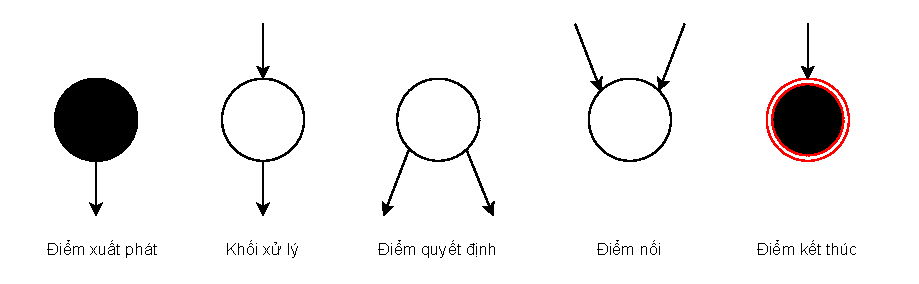
\includegraphics[width=1\columnwidth]{figures/c2/c2_cfg_point.drawio.pdf}
  \centering
  \caption{Các thành phần cơ bản trong đồ thị CFG.}
  \label{img:c2_cfg_point}
\end{figure}

Đồ thị luồng điều khiển bao gồm các thành phần chính là điểm xuất phát, khối xử lý, điểm quyết định, điểm nối và điểm kết thúc.
Trong hình \ref{img:c2_cfg_point}, \textbf{điểm xuất phát} và \textbf{điểm kết thúc} biểu thị điểm bắt đầu và kết thúc của chương trình, lần lượt được thể hiện bằng hình tròn đặc và hình tròn đặc có viền.
\textbf{Khối xử lý} tượng trưng cho các câu lệnh gán, khai báo và khởi tạo, được thể hiện bằng hình tròn rỗng.
\textbf{Điểm quyết định} biểu thị các câu lệnh điều kiện trong các khối lệnh rẽ nhánh, được thể hiện bằng hình tròn rỗng với hai cạnh đi ra.
\textbf{Điểm nối} biểu thị các câu lệnh thực hiện ngay sau các lệnh rẽ nhánh, có hai cạnh nối đến, được thể hiện bằng hình tròn rỗng.

\begin{figure}[H]
  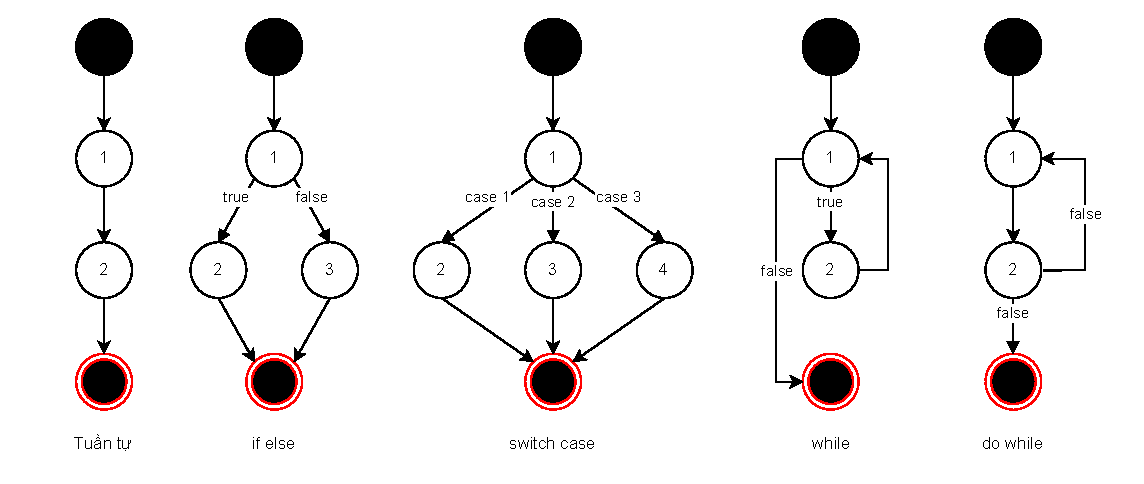
\includegraphics[width=1\columnwidth] {figures/c2/c2_cfg_line.drawio.pdf}
  \centering
  \caption{Các cấu trúc điều khiển phổ biến trong các ngôn ngữ lập trình.}
  \label{img:c2_cfg_line}
\end{figure}

Hình \ref{img:c2_cfg_line} mô tả các cấu trúc điều khiển phổ biến có trong các ngôn ngữ lập trình được biểu diễn dưới dạng đồ thị CFG, bao gồm có cấu trúc điều khiển tuần tự, if else, switch case, while và do while.

\subsection{Đồ thị phụ thuộc chương trình}

% The PDG makes explicit both the data and control dependences for each operation in a program. Data dependence graphs have provided some optimizing compilers with an explicit representation of the definition-use relationships implicitly present in a source program [31, 361]. A control flow graph [1, 31] has been the usual representation for the control flow relationships of a program; the control conditions on which an operation depends can be derived from such a graph. An undesirable property of a control flow graph, however, is a fixed sequencing of operations that need not hold. The program dependence graph explicitly represents both the essential data relationships, as present in the data dependence graph, and the essential control relationships, without the unnecessary sequencing present in the control flow graph.’ These dependence relationships determine the necessary sequencing between operations, exposing potential parallelism.

% The PDG represents a program as a graph in which the nodes are statements and predicate expressions (or operators and operands) and the edges incident to a node represent both the data values on which the node’s operations depend and the control conditions on which the execution of the operations depends

Đồ thị phụ thuộc chương trình (Program Dependence Graph) \cite{ferrante1987program} là đồ thị có hướng thể hiện hai khía cạnh của chương trình, phụ thuộc điều khiển và phụ thuộc dữ liệu.
Một nút đại diện cho các mệnh đề hoặc mệnh đề điều kiện, một cạnh thể hiện mối quan hệ phụ thuộc điều khiển hoặc phụ thuộc dữ liệu giữa các nút.
Mệnh đề mà một nút đại diện có được thực thi hay không phụ thuộc vào các cạnh điều kiện điều khiển trỏ tới nút, giá trị của các biến mà mệnh đề sử dụng phụ thuộc vào các cạnh phụ thuộc dữ liệu trỏ tới nút đó.
Lưu ý rằng cạnh phụ thuộc điều khiển không giống như cạnh luồng điều khiển của đồ thị CFG.
Cạnh phụ thuộc điều khiển chỉ thể hiện điều kiện để mệnh đề của một nút được thực thi, không thể hiện thứ tự thực thi của mệnh đề giữa các nút.

\begin{figure}[H]
  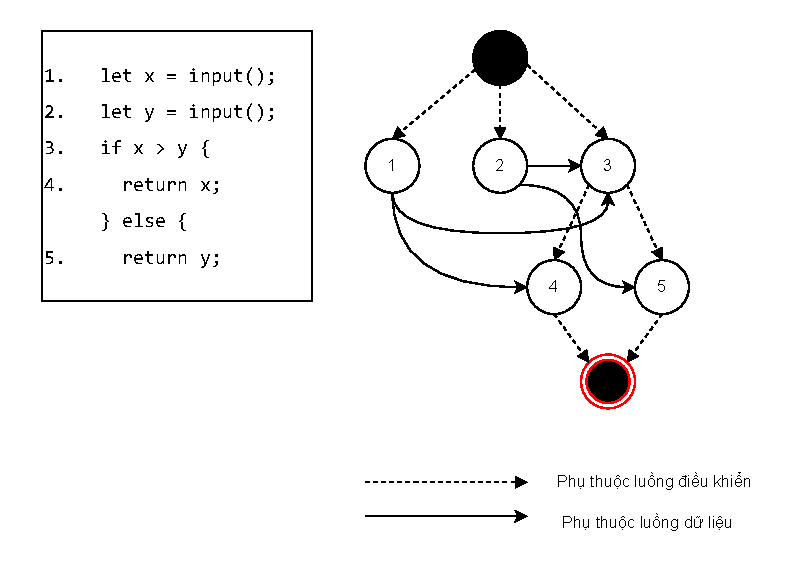
\includegraphics[width=1\columnwidth]{figures/c2/c2_pdg.drawio.pdf}
  \centering
  \caption{Ví dụ về đồ thị PDG.}
  \label{img:c2_pdg}
\end{figure}

Hình \ref{img:c2_pdg} biểu diễn ví dụ về một đồ thị PDG với cấu trúc điều kiện if else trong ngôn ngữ Rust, các cạnh nét đứt biểu diễn phụ thuộc điều khiển và các cạnh nét liền biểu diễn phụ thuộc dữ liệu.

\subsection{Đồ thị thuộc tính mã nguồn}

Đồ thị thuộc tính mã nguồn (Code Property Graph) \cite{yamaguchi2014modeling} là một dạng đồ thị biểu diễn mã nguồn hợp thành từ cây AST, đồ thị CFG và đồ thị PDG.
Đồ thị chứa các thông tin về cấu trúc cú pháp, luồng điều khiển và phụ thuộc dữ liệu trong chương trình
Đồ thị CPG tạo ra một lớp biểu diễn trung gian cho mã nguồn mà không bị phụ thuộc vào ngôn ngữ lập trình cụ thể.
Các nút đại diện cho các thành phần như hàm, biến, lớp và các cạnh đại diện cho mối quan hệ giữa chúng như lời gọi hàm, sự gán giá trị, quan hệ cha con hay tham chiếu.
Mỗi nút, cạnh đều có các thuộc tính, mỗi thuộc tính có giá trị riêng.
Đồ thị CPG được ứng dụng để tìm kiếm lỗ hổng trong mã nguồn, phát hiện sao chép mã nguồn bằng học máy, học tăng cường \cite{zhou2019devign, han2023bjxnet}.
Hình \ref{img:c2_cpg_yamaguchi} minh họa một đồ thị CPG cho mã nguồn C \cite{yamaguchi2014modeling}.

% \begin{figure}[H]
%   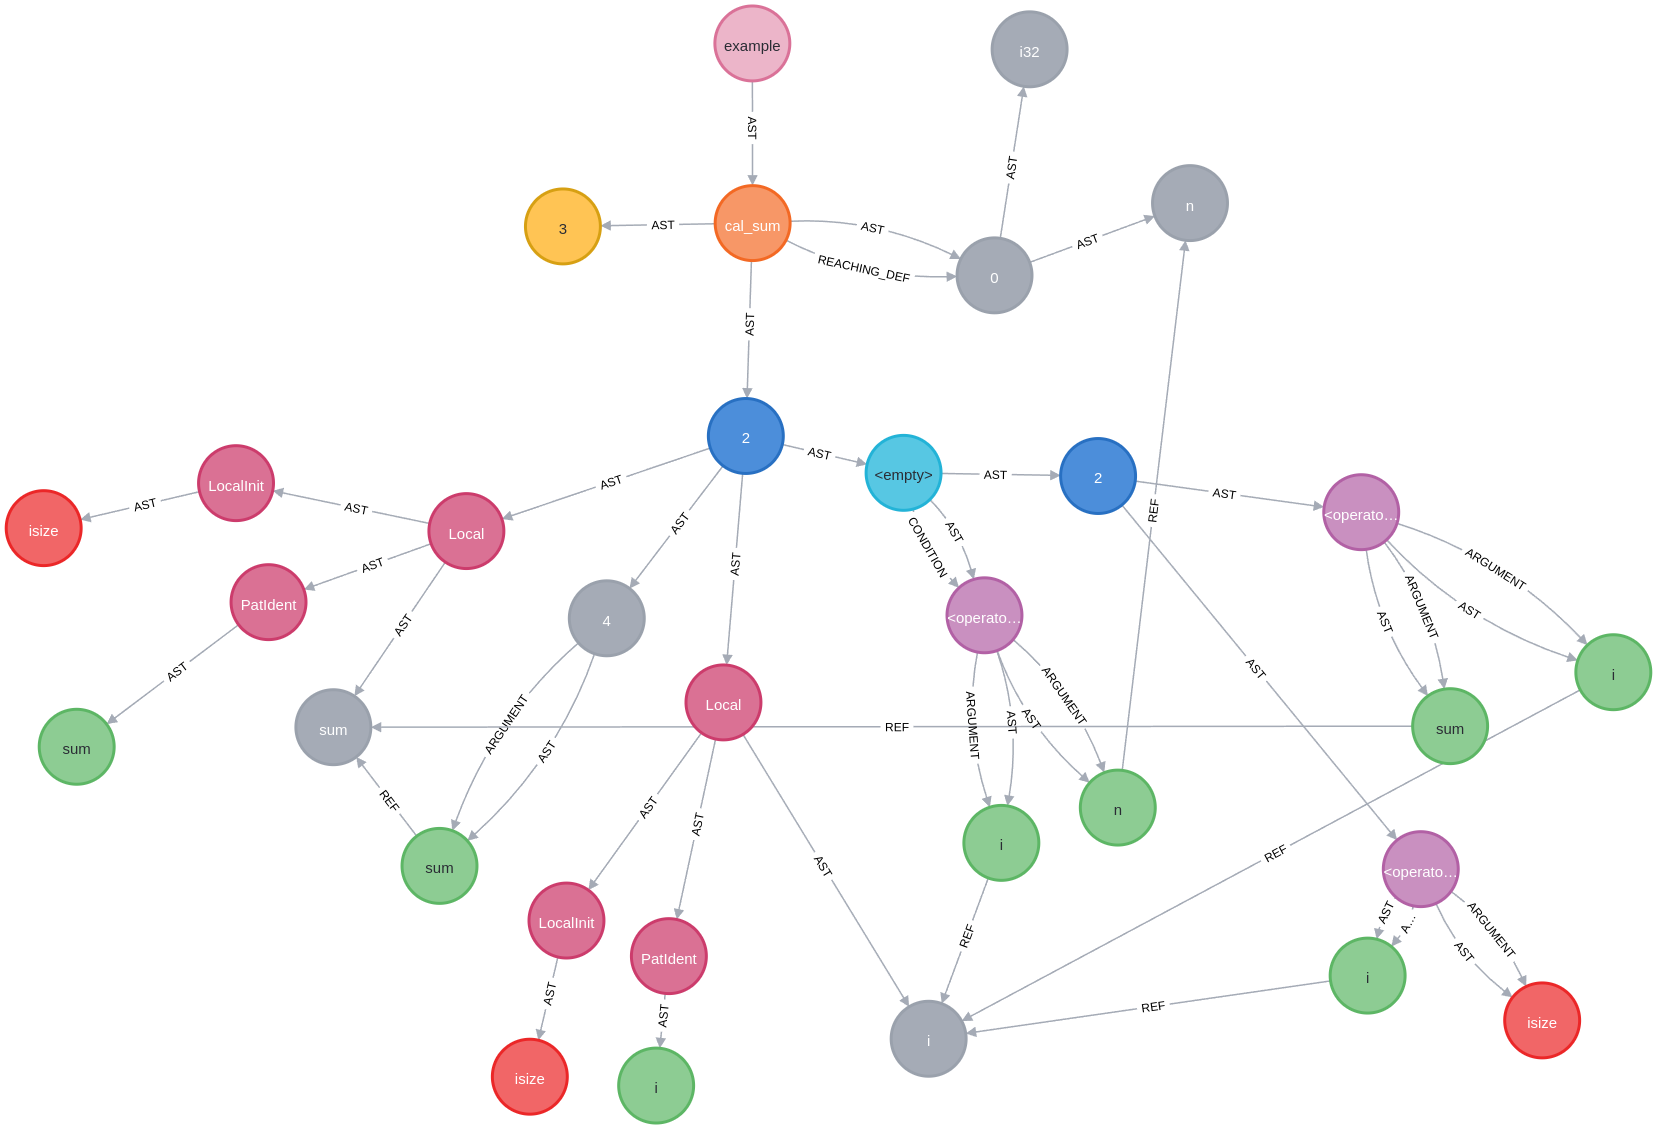
\includegraphics[width=1\columnwidth]{figures/c2/c2_cpg.png}
%   \centering
%   \caption{Ví dụ đồ thị CPG.}
%   \label{img:c2_cpg}
% \end{figure}

\begin{figure}[H]
  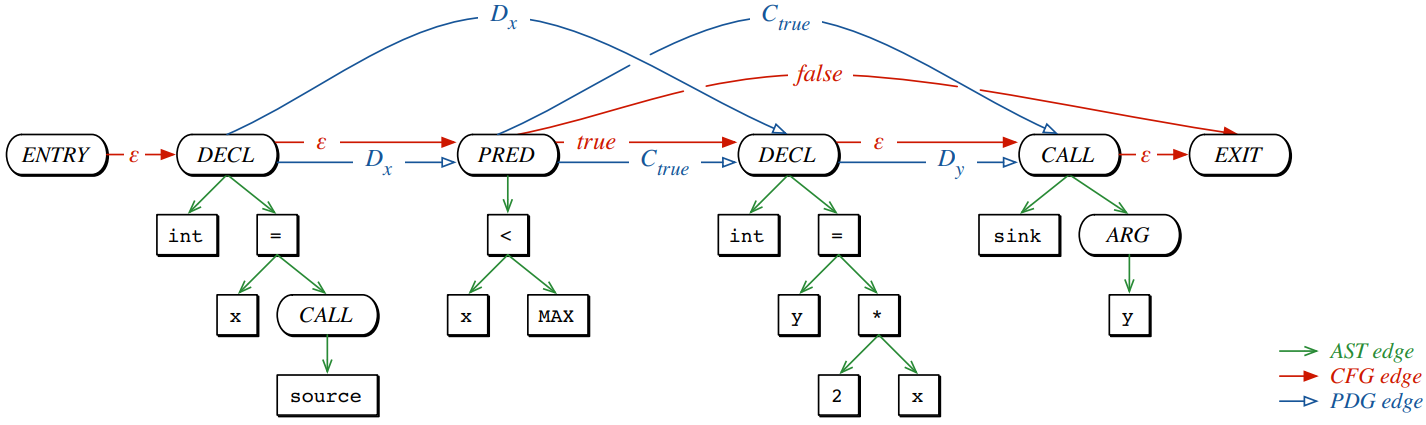
\includegraphics[width=1\columnwidth]{figures/c2/c2_cpg_yamaguchi.png}
  \centering
  \caption{Minh họa đồ thị CPG \cite{yamaguchi2014modeling}.}
  \label{img:c2_cpg_yamaguchi}
\end{figure}


% \begin{listing}[H]
% \begin{minted}[mathescape, breaklines, frame=lines, framesep=2mm, baselinestretch=1.2, fontsize=\footnotesize, linenos]{rust}
% fn cal_sum(n: i32) {
%   let mut sum = 0;
%   let mut i = 1;
%   while i <= n {
%       sum += i;
%       i += 1;
%   }
%   return sum;
% }
% \end{minted}
% \caption{Mã nguồn đầy đủ cho đồ thị CPG hình \ref{img:c2_cpg}.}
% \label{code:c2_cpg}
% \end{listing}
